% -*-coding: utf-8-*-
\startprefacepage

Построение минимальной филогенетической сети является важной задачей филогенетики.
Филогенетическая сеть используется для представления эволюционных взаимосвязей между различными биологическими видами в ретикулярной модели эволюции.
В ретикулярной (сетчатой) модели эволюции, в отличие от классической (древовидной) модели, присутствует горизонтальный перенос генов, а также гибридизация между видами, что не позволяет использовать более простые структуры, такие как филогенетические деревья.
Филогенетические сети активно исследуются в настоящее время~\cite{huson2010phylogenetic, morrison2011introduction, 
nakhleh2011evolutionary}.

Хотя существует несколько формальных определений филогенетических сетей, в данной работе рассматриваются только гибридизационные сети~\cite{semple2006hybridization, chen2010hybridnet}.
Исходными данными для построения гибридизационной сети является набор из нескольких филогенетических деревьев, построенных на одном и том же множестве таксонов.
Каждое филогенетическое дерево представляет собой эволюционную историю какого-то гена.
Деревья могут иметь различную топологию из-за наличия ретикуляций.
Задача состоит в том, чтобы построить гибридизационную сеть с минимальным количеством вершин, содержащую в себе каждое из исходных деревьев как подграф.

Большинство алгоритмов для построения гибридизационных сетей основаны на эвристиках и не гарантируют точный результат~\cite{wu2013algorithm, park2012murpar}.
Кроме того, многие алгоритмы не могут работать более чем с двумя деревьями.

В данной работе представлен новый способ построения минимальной гибридизационной сети, основанный на сведении к задаче о выполнимости булевой формулы (SAT), гарантирующий точный результат.

Подходы, основывающиеся на сведении к задаче SAT, успешно применяются для решения различных задач, в том числе для задач филогенетики~\cite{bonet2009efficiently}, построения конечных автоматов~\cite{heule2010exact} и верификации~\cite{biere2003bounded}.
Это обусловлено тем, что современные SAT-солверы хорошо оптимизированы, и способны успешно справляться с формулами из десятков тысяч переменных за несколько минут.

\begin{figure}[t]
  \centering
  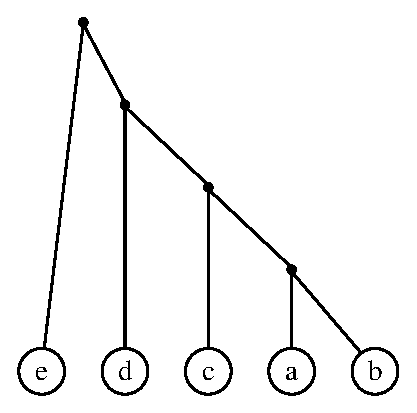
\includegraphics[width=1.4in]{img/inp1.eps}
  ~~~
  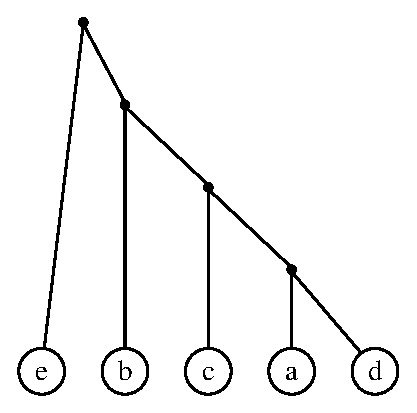
\includegraphics[width=1.4in]{img/inp2.eps}
  ~~~
  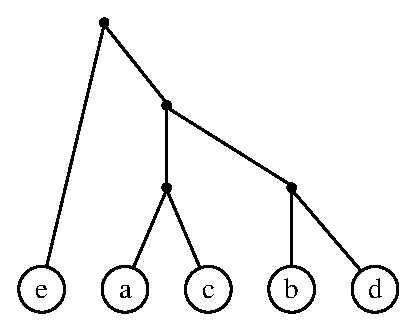
\includegraphics[width=1.4in]{img/inp3.eps}
  \caption{Example of three gene trees over the set of taxa \{a, b, c, d, e\}.}
  \label{input-example}
\end{figure}

\begin{figure}[t]
  \centering
  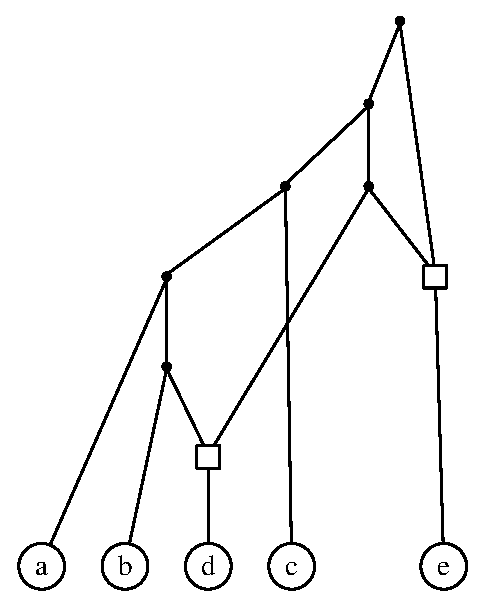
\includegraphics[width=1.4in]{img/ans.eps}
  ~~~~~~
  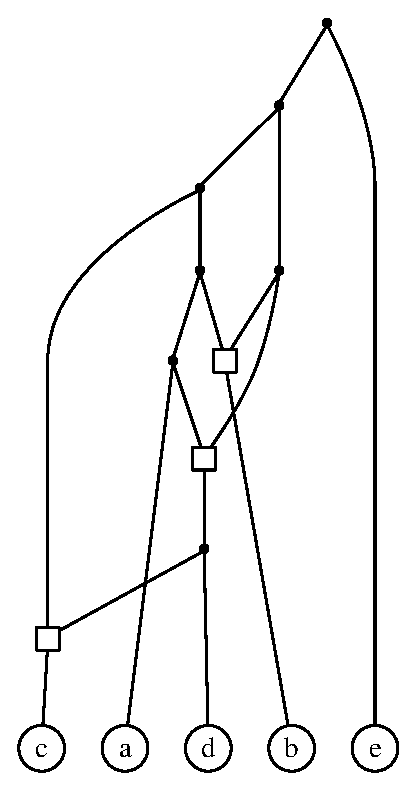
\includegraphics[width=1.4in]{img/ans3.eps}
  \caption{Possible hybridization networks for the trees from Fig.~\ref{input-example} with two and three hybridization events respectively. Reticulation nodes are shown as boxes.}
  \label{network-example}
\end{figure}